\documentclass[12pt]{thesis}


% The default font is Computer Modern Roman for text and math. Uncomment
% one of the following to choose a different font set.
% \usepackage{mathptmx} % Times New Roman with math fonts
% \usepackage{newcent}  % new century schoolbook font
% \usepackage{bookman}  % bookman font
% \usepackage{fourier}  % Utopia (text) and Fourier (math) font
\usepackage{times}
\usepackage{mathptm}
  
\usepackage{graphicx}
\usepackage{rotating}
\usepackage{makeidx}
\usepackage{subfig}

%% Uncomment the following two lines and comment out the third one
%% if you want to use the Chicago Manual based bibliography.
% \usepackage{thesiscitations}
% \bibliographystyle{thesis}
\bibliographystyle{ieeetr}

%% Change ieeetr in the previous line to any bibliography style you
%% like

%% Uncomment next line if you want chapter titles centered (not
%% approved by SDSMT graduate school)
% \centertitles

%% Uncomment next line to print a double-spaced draft version
% \dsdraft

%% Uncomment next line to print a single-spaced draft version
% \ssdraft

%% Uncomment next line if you are using makeindex to create an index
% \makeindex

\doctype{thesis}
% Title is a work in progress
\title{MIMIC: Machine Intelligence Mastery Imitation Control}
\author{Kyle MacMillan}
\degree{Master of Science in Computational Science and Robotics}
\defensedate{December XX, 2019}
\gradyear{2019}
\department{Computer Science}

% The following commands add a signature line for each person who needs
% to sign the thesis/dissertation
\signatureline{Major Professor --- Larry Pyeatt, Ph.D., Department of
  Computer Science}

\signatureline{Graduate Division Representative --- E.\ Nigma, Ph.D.,
  Department of Philosophy}

\signatureline{Committee Member --- Chip Munk, Ph.D., Department of
  Zoology}

\signatureline{Committee Member --- Gail Force, Ph.D., Department of
  Meteorology }

\signatureline{Head of the Computer Science Department --- Jeff McGough, Ph.D.}

\signatureline{Dean of Graduate Education --- Maribeth Price}

\begin{document}

\maketitle

%% Comment the next line to remove the copyright notice.  Read the
%% section on copyright in the Thesis and Dissertation Writing
%% Instructions.
\makecopyright % copyright must go BEFORE \preliminaries


\preliminaries


\begin{abstract}
TBD
\end{abstract}

%% Uncomment the following if you want acknowledgements
\begin{acknowledgments}
I would like to thank my advisor, Dr.\ Larry Pyeatt for all of the advice and 
guidance he has given me. Also my wife, who helped in an uncountable number of 
ways.
\end{acknowledgments}

\tableofcontents

\listoftables

\listoffigures

%% Uncomment following lines if you want a list of symbols
% \begin{listofsymbols}
% \begin{tabular}{ll}
%   $\mathcal{G}_t$ & Gnat\\
%   $\mathcal{G}_u$ & Gnu
% \end{tabular}
% \end{listofsymbols}

%% Uncomment following lines if you want a list of keywords
% \begin{listofkeywords}
% \noindent Gnat, Gnu
% \end{listofkeywords}

%% Uncomment following lines if you want a dedication
% \begin{dedication}
% In loving memory of 
% my grandmother.
% \end{dedication}

%% Uncomment following lines if you want a preface
% \begin{preface}
% Before we begin, just let me say one thing.
% Gnat and gnu are both begin with ``gn,'' and
% the purpose of this work was to see if there
% are any other resemblances.
% This thesis has taken 45 years of work, and
% I don't have much time left in this world, but it
% has been worth it.  When the time comes,
% I would like to die as my grandmother did, peacefully in
% her sleep, not screaming like the passengers in her car.
% \end{preface}


\body


\chapter{Introduction}
Up to this point the majority of artificial intelligence in games have been 
made by humans designing an algorithmic response to player input or game 
mechanics\cite{NestedIF}. The method of creating an artificial intelligence for 
a game has improved over time\cite{AdvancedIF} but is still essentially humans 
developing these systems. There is nothing wrong with humans designing 
artificial intelligence in games but is there any way to leverage machine 
learning to create an equivalent, or better, gaming experience that is less 
prone to programmer error?

We design artificial intelligence in games to behave as humans, or in the case 
of games involving other creatures, how we imagine they would behave. This 
paper proposes utilization of humans \textit{playing} a game to train an 
artificial intelligence to play as the human does. This approach could yield 
many benefits:

\begin{itemize}
    \item Reduced developer workload
    \item Reduction in exploitable behavior
    \item Enhanced immersion
    \item Greater variety in game play
\end{itemize}

In a first-person shooter scenario developers must design a system that teaches 
agents how to navigate, attack, resupply, and coordinate. While that list is 
short, the amount of time required is extensive. They must then tweak behaviors 
to keep games fun\cite{Fairness}. By taking a machine learning approach to 
training artificial intelligence behavior the workload is considerably reduced 
and the process is largely reusable. 

Humans are adept at finding exploits within a system. Players tend to notice 
artificial intelligence pathing flaws and use them to their advantage. The 
reason an agent will behave in an exploitable way is because developers and 
testers can only test so many possibilities under tight time constraints. A 
game released to millions of people allows for many more possibilities to be 
tested. 

That exploitable or erratic behavior leads to a disruption in player immersion. 
If the agent runs into a wall and struggles to path plan to a player it 
disrupts the game for the player. Another time this causes problems is when 
missions/quests ask the player to assist someone moving from point \textit{A} 
to \textit{B}. The agent usually does not behave in an intelligent, expected, 
or human-like behavior. 

In most cases one ``skeleton'' from a game behaves in the same manner as any 
other in the game because they run a ``skeleton'' agent. The difficulty of the 
agent can be tweaked, it's abilities can be tweaked, or it's decision making 
can be tweaked, but all of those require considerable effort on the part of the 
engineers.

This paper poses the question: Can we mimic human behavior in a three 
dimensional space shooter such that it is distinguishable between two players, 
while being indistinguishable from human-play?



\chapter{Previous Work}
Reinforcement Learning for games was really brought into light by the DeepMind 
team's work on Atari games\cite{Atari_DM}. Work in this field has been 
surprisingly minimal and that is likely due to the difficulty in training 
reinforcement learning agents. On a simple DQN DeepMind trained for 10 million 
frames and 100 epochs, with epochs corresponding to 30 minutes of training time. 
Roughly 50 hours of training time on top-of-the-line equipment. DeepMind later 
released the StarCraft 2 Learning Environment (SC2LE)\cite{SC2LE}. Where it 
took over 3 weeks to train on an Nvidia GTX-1060. Further progress and more 
elaborate networks/algorithms required \textit{200 years} of training which 
took a week on their server farm.

This barrier to entry is quite steep and has kept papers related to 
reinforcement learning, in games, sparse.

The attempts that have been made were to make the agent equal to or better than 
humans in \textit{score}. Score is a quantitative way to assess the progress of 
your agent, and is well suited for that task. Even the more recent papers such 
as Electronic Arts' SEED\cite{EA_SEED} focused on maximizing score. They stated 
the average expert human player scored 47, whereas their agent scored 100. The 
focus of all papers is on maximization of score. This paper aims for agent 
scores that are on-par with the humans that trained it.

The paper that most relates as a previous work was for general video game 
playing\cite{Human-Like}. Their solution approached the problem using a variant 
of Monte Carlo Tree Search. They also used simplified versions of the games, 
what is knows as Video Game Definition Language (VGDL). VGDL allows for a much 
simpler game as can be seen in Table \ref{tab:vgdl_as}. The agent doesn't have 
to determine if it should open a map, use an item, etc. 

\begin{table}
  \caption{VGDL Action Space}
  \begin{center}
    \begin{tabular}{ | c | c | c | c | c | }
      \hline
      \bf Game & \bf Movement & \bf No Action & \bf Other & \bf Total \\ \hline
      Aliens & 2 & 1 & 1 & \bf 4 \\ \hline
      PacMan & 4 & 1 & 0 & \bf 5 \\ \hline
      Zelda & 4 & 1 & 1 & \bf 6 \\
      \hline
    \end{tabular}
  \end{center}
  \label{tab:vgdl_as}
\end{table}




\chapter{Methods}
\begin{table}
  \caption{MIMIC Single Action Space}
  \begin{center}
    \begin{tabular}{ | c | c | }
      \hline
      \bf Name & \bf Actions \\ \hline
      \hline
      None & 1 \\ \hline
      Thrust & 3 \\ \hline
      % increase, decrease, no change
      Look & 361 \\ \hline
      Attack & 1 \\ \hline
      \bf Total & \bf 365 \\
      \hline
    \end{tabular}
  \end{center}
  \label{tab:mimic_as}
\end{table}


\section{Game Environment}
For the purpose of this paper a new game environment was created. A custom 
environment was created because there is a need to control certain aspects of 
the game such as models, resolution, data sample rate, physics, and actions. 

The game environment recognizes the actions listed in Table \ref{tab:mimic_as}. 
Modern games tend to require multiple actions simultaneously such as firing and 
looking in a direction and this environment allows for that as well. To make 
training simpler user input is collected at predetermined, regular interval of 
50 Hz. % https://docs.unity3d.com/ScriptReference/MonoBehaviour.FixedUpdate.html
The environment uses classical mechanics, meaning objects in motion will stay in 
motion. Enemy ships are red and their projectiles are red; friendly ships and 
projectiles are green. Engine control has \textit{forward}, \textit{reverse}, 
or \textit{no change}. Forward and reverse apply acceleration to the vessel 
while no change will maintain the current speed due to the physics method 
chosen. Vessels require five shots to be destroyed and vessels can shoot up to 
four times per second.

\begin{table}
  \caption{Agent Input}
  \begin{center}
    \begin{tabular}{ | c | }
      \hline
      Health \\ \hline
      Speed \\ \hline
      Action \\ \hline
      Look \\ \hline
      Screen \\ \hline
    \end{tabular}
  \end{center}
  \label{tab:agent_input}
\end{table}

% Unity FixedUpdate for regular interval readings of actions
% Investigate Poisson Distribution
% Investigate Beta Negative Binomial Distribution
\section{Training}
Each player spends five minutes getting used to the game. The player then plays 
$N$ % 10?
scenarios. These scenarios train the agent to play like that person. $J$ 
scenarios are used for training and $N - J$ are used to verify. After 
the training there are $M$ % 4?
test scenarios. 

Table \ref{tab:mimic_as} shows that there are 365 single actions for the agent. 
Multi-actions are possible such as looking, changing thrust, and firing. This 
leads to a total action space of: $ 3 \times 361 \times 2 + 1 = 2167$

As a person plays the game all input is recorded and saved in files to be fed 
to the agent during training. The agent receives the information listed in 
Table \ref{tab:agent_input}. \textit{Health}, \textit{speed}, and 
\textit{action} are stored in a contiguous manner, so there is no need for a 
time stamp. 
% I need to nail-down the look mechanics first. Looking is usually on a curve 
% depending on how far from center the mouse makes it.
% \textit{Look} utilizes normalized $\sin\(degree\)$ that a player looked at in 
% that time step. If a player did not move the mouse then the 
The screen data is recorded in $128 \times 128$ pixels and piped through 
$N$ convolutions. 
% Unity screen capture http://answers.unity.com/answers/1296574/view.html

\section{Validation}
To verify that the algorithm performed in a human-like manner several 
Turing-test-like studies were used. 

\subsection{Side-by-side}
Users were shown $M$ side-by-side test scenarios and were asked to label each 
as either human or agent. Location of human and agent videos was randomized for 
each scenario. The goal of this was to see if agents were indistinguishable 
from humans.

\subsection{Pick a player}
Users were shown an agent in the top video and two players in the bottom videos. 
Users were then asked to identify which of the two videos were being 
represented by the agent. The purpose of this was to determine if the agent 
appropriately represented the player.



\chapter{Results}
My research had fabulous results. I will now tell you about
the results, because they are the best!  You are not going
to believe how good my results are.

\section{Visual comparison}
%\index{comparison!visual}

\begin{table}
\caption{Results of visual comparison studies.}
\begin{center}
  \begin{tabular}{|c|c|}
    \hline
    \bf Categories & \bf Percent Correct\\
    \hline
    \hline
    insect/mammal & 76\\
    \hline
    gnat/gnu & 69\\
    \hline
  \end{tabular}
\end{center}
\label{table:comp1}
\end{table}

The first test that I performed was a visual comparison of gnats and
gnus.  First, I went on the internet and downloaded several thousand
pictures of gnats, and one picture of a gnu.  Then, I had two
volunteers compare them and categorize them as insect
%\index{insect}
or mammal.
%\index{mammal}
Next, I selected another group of volunteers and
had them classify the photographs as either gnat or gnu.


\begin{sidewaysfigure}
\begin{center}
\subfloat{\resizebox{0.45\textheight}{!}{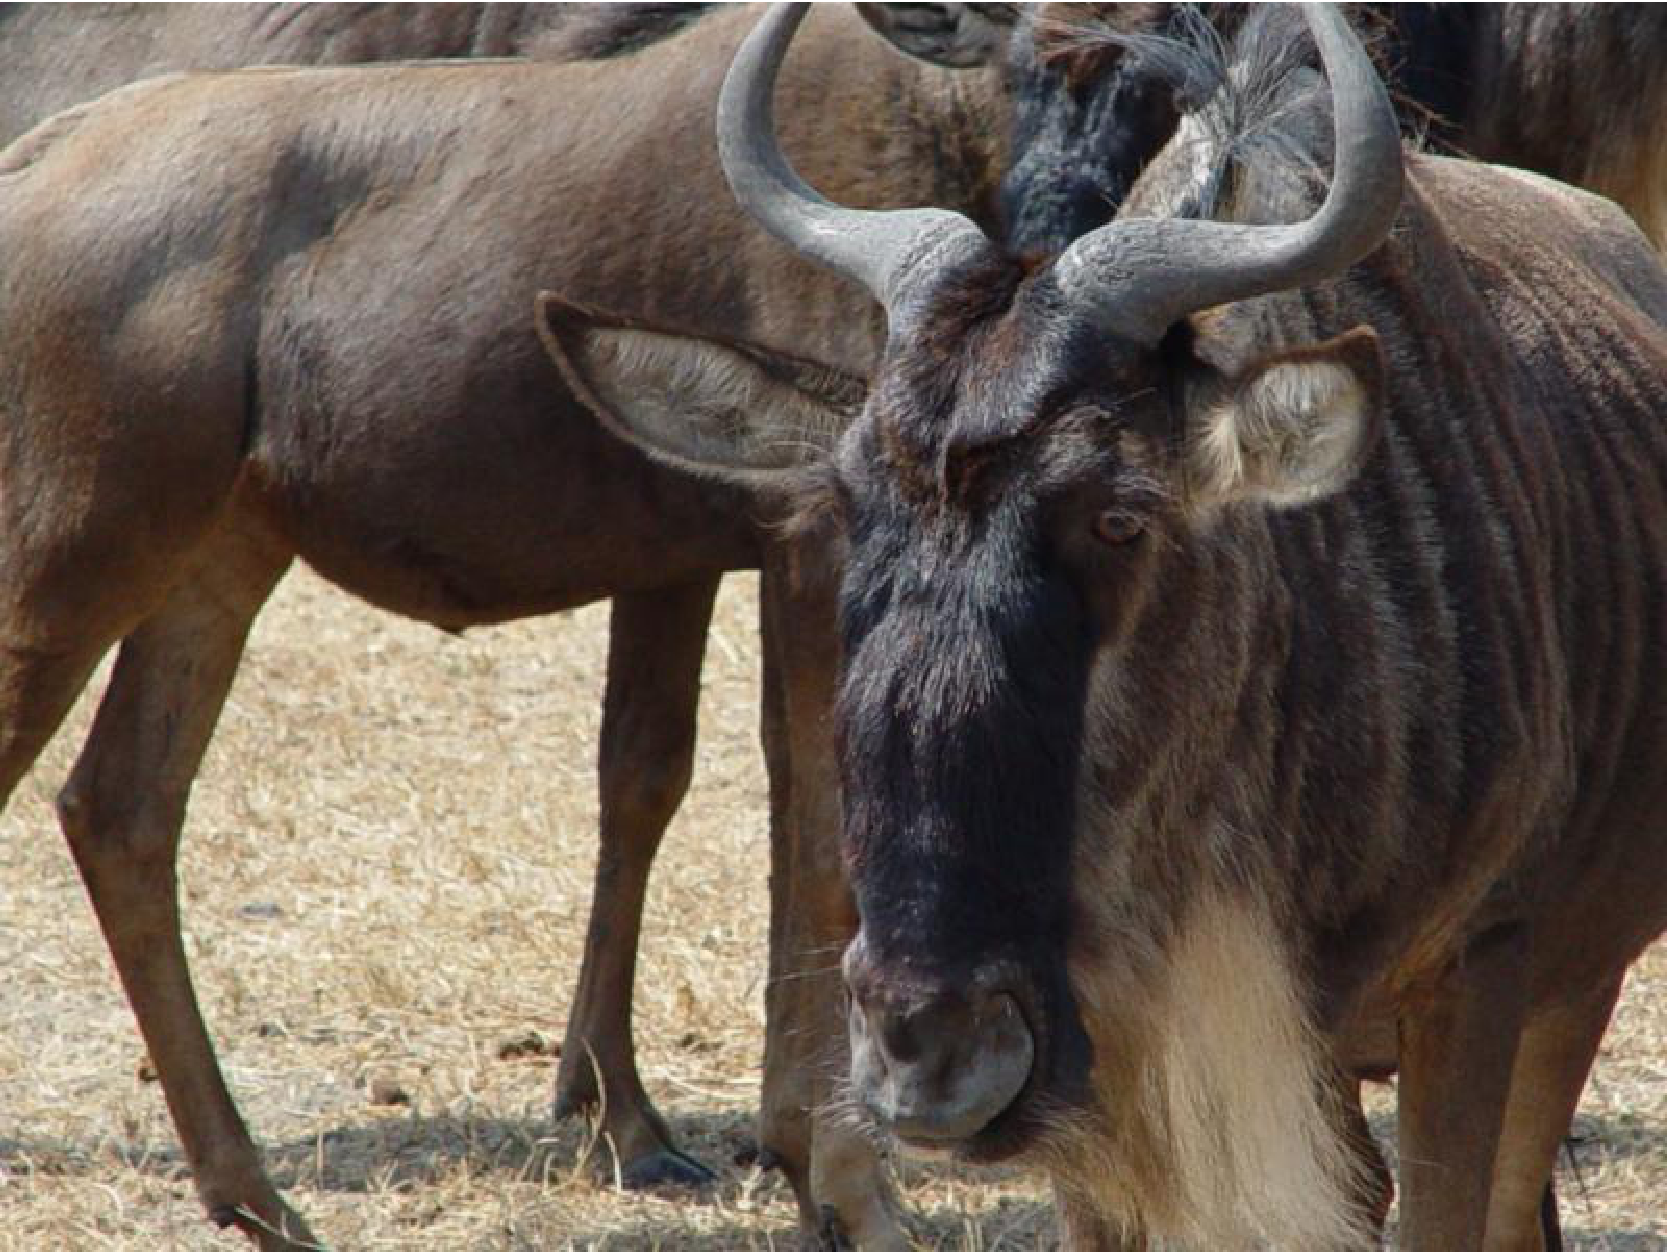
\includegraphics{images/gnu.pdf}}}
\subfloat{\resizebox{0.45\textheight}{!}{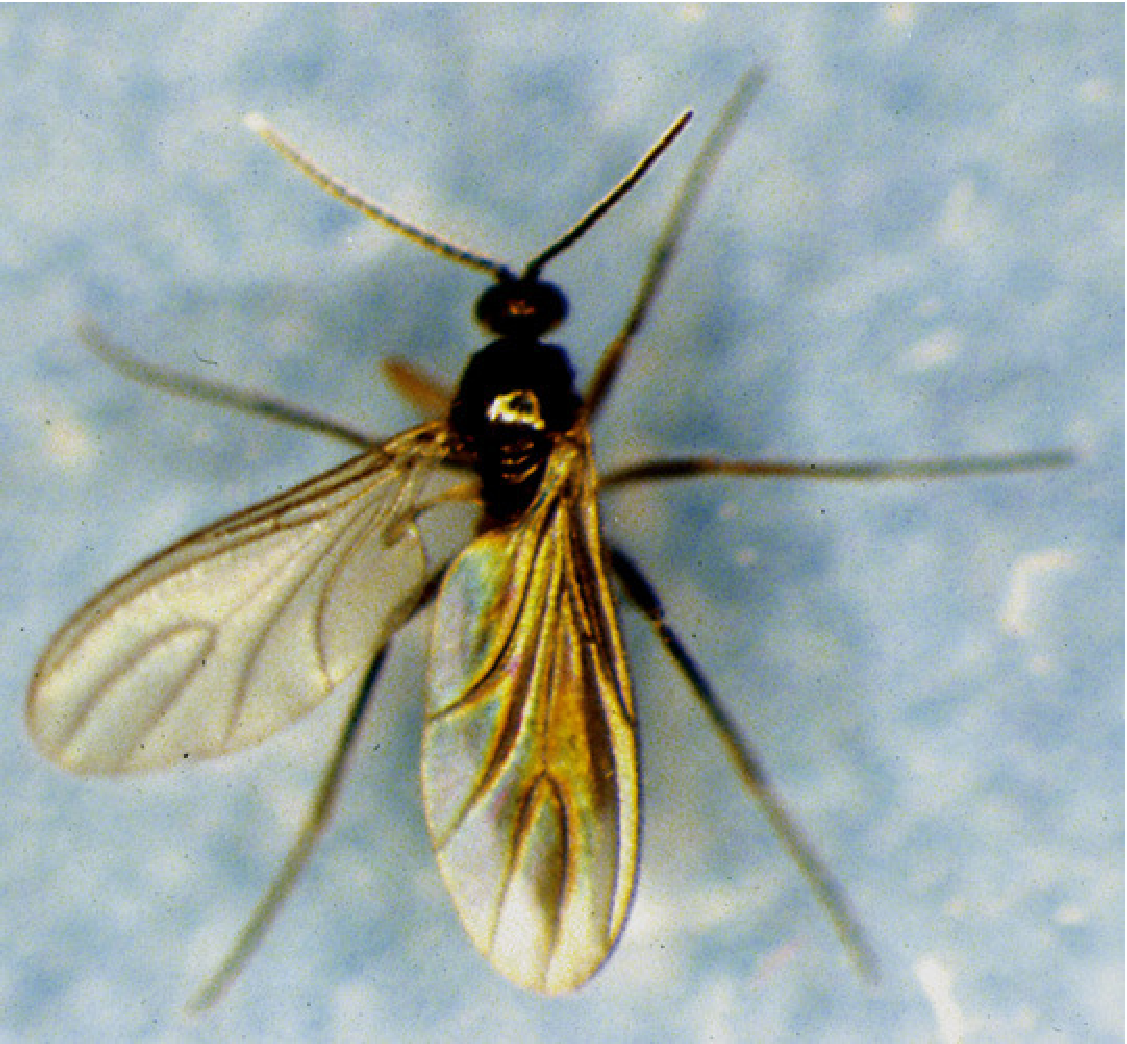
\includegraphics{images/gnat.pdf}}}
\end{center}
\caption{Photographs of a gnu (left) and a gnat (right).}
\label{figure:photos}
\end{sidewaysfigure}

The results of this comparison are shown in Table~\ref{table:comp1}.
As can be seen, both volunteers (myself and my advisor) were able to
correctly classify most of the photographs.  As a result, we gave each
other little gold stars.
For those who are interested, Figure~\ref{figure:photos} shows the gnu
photograph and one of the gnat photographs.

\section{Comparison by Size}
\index{comparison!size} As can be seen from
Figure~\ref{figure:photos}, photographs of gnats are slightly larger
than photographs of gnus.  This leads us to believe that
statistically, gnats are slightly larger than gnus.  Mathematically,
we express this as follows:
\begin{equation}
S(\mathcal{G}_t) > S(\mathcal{G}_u) \forall
\mathcal{G}_t,\mathcal{G}_u,
\end{equation}
where $\mathcal{G}_t$ is a photograph of a gnat and $\mathcal{G}_u$ is
a photograph of a gnu.  The $S()$ function calculates the ``size'' of
the photograph.

\chapter{Conclusions}

Well, there you have it.  My advisor and I were able to tell the
difference between a photograph of a gnat and a gnu most of the time.
Also, gnats are larger than gnus, and therefore, they are
significantly different.

In the future, we plan to apply the techniques developed in this
research to answer the age old question of whether dogs and ducks are
the same thing.

\supplementaries


\bibliography{macmillan}


\begin{appendices}

\appendix{Appendix A} Well, I really have nothing more to say,
but wanted to have an appendix.

\end{appendices}

%% Uncomment the following lines if you want to create a glossary
% \begin{gloss}
% I don't have a glossary either, but this is what the page would look
% like if I did.
% \end{gloss}


%% uncomment following lines if you want to create a list of abbreviations
% \begin{abbreviations}
% gnu is abbreviated to gnu\\
% gnat is abbreviated to gnat
% \end{abbreviations}

%% uncomment next line if you used makeindex to make an index
%\printindex

\begin{vita}

  
  Format the vita page according to the following graduate school requirements:

A vita page, not over one page in length, is to be included as the
last page of all theses and dissertations deposited in the Devereaux
Library. The vita is to be written in the third person using
professional style and could contain the following information
(although you may wish to omit A and B if concerned about identity
theft):
\begin{enumerate}[label=\Alph*.]
\item Place and date of birth.

\item Place and date of high school graduation.

\item Place and date of college graduation—with degree and major.

\item Place and date of receipt of master’s degree—with major.

\item Vocational and professional experience (not summer jobs)—including dates, nature of position, and school or organization.

\item Military experience, with indication of professional relevance—if any.

\item Scholarly publications, exhibits of creative work, membership in professional organizations and honorary societies.
\end{enumerate}
  

\end{vita}



\end{document}
